% !TeX spellcheck = en_EN-English
\documentclass[a4paper]{article}
\usepackage[english]{babel}
\usepackage[utf8]{inputenc}
\usepackage[T1]{fontenc}
\usepackage{a4wide}
\usepackage{amsmath}
\usepackage{amsfonts}
\usepackage{amssymb}
\usepackage{mathrsfs}
\usepackage[small,bf]{caption}
\usepackage{subcaption}
\usepackage{xcolor}
\usepackage{graphicx}
\usepackage{enumerate}
\usepackage{hyperref}
\usepackage{tikz}

\let\origfontsize\fontsize
\def\fontsize#1#2{\origfontsize{11}{14.5}}

\xdef\mypath{C:/Users/majko/Desktop/weather_prediction/images}

\pagestyle{empty}
\setlength{\parindent}{0pt}

\newenvironment{modenumerate}
{\enumerate\setupmodenumerate}
{\endenumerate}

\newif\ifmoditem
\newcommand{\setupmodenumerate}{%
	\global\moditemfalse
	\let\origmakelabel\makelabel
	\def\moditem##1{\global\moditemtrue\def\mesymbol{##1}\item}%
	\def\makelabel##1{%
		\origmakelabel{##1\ifmoditem\rlap{\mesymbol}\fi\enspace}%
		\global\moditemfalse}%
}

\renewcommand{\thesubsection}{\alph{subsection})}

\makeatletter
\def\@seccntformat#1{%
	\expandafter\ifx\csname c@#1\endcsname\c@section\else
	\csname the#1\endcsname\quad
	\fi}
\makeatother
\def\checkmark{\tikz\fill[scale=0.4](0,.35) -- (.25,0) -- (1,.7) -- (.25,.15) -- cycle;} 
\begin{document} 
	
	\pagenumbering{arabic}
	\pagestyle{plain}
	
	\begin{center}
		\sc\large
		ML Project
		\\
		Determining whether weather is good for picnic 
	\end{center}
	
	Author: Marián Kravec
	
	\section{Introduction}
	
	In this project, our objective is to develop models capable of accurately assessing whether particular weather conditions, such as temperature or humidity, are conducive to an enjoyable picnic experience.
	\\
	
	Our primary aim does not involve exhaustively testing numerous models, optimizing their parameters, and identifying a singular best model. Instead, our focus is directed towards more intriguing pursuits, such as comparing the outcomes of analogous models or experimenting with techniques designed to enhance overall model performance.
	\\
	
	The project will unfold in three main segments, excluding the section introducing the data. Initially, we will undertake a comparative analysis of three implementations of the Support Vector Machine, specifically the Support Vector Classifier. This comparison will primarily involve default parameters, allowing us to identify the most effective classifier for our weather data.
	\\
	
	In the second phase, our focus will shift to Neural Networks, with a specific emphasis on transfer learning. Our objective is to explore whether incorporating transfer learning techniques contributes to enhancing the performance of our model.
	\\
	
	The concluding part centers around unsupervised learning. In this stage, we will experiment with various clustering algorithms to discern if any of them exhibit a similar data partitioning as the labeled picnic weather categories.
	\\
	
	The code utilized for generating the results in this project is accessible in the GitHub repository, which can be found at the following link: \url{https://github.com/MarianK-py/projekt_stojove_ucenie}.
	
	\newpage

	\section{Data}
	
	\subsection{Source and content}
	Data used for classification and prediction are from Kaggle (\url{https://www.kaggle.com/datasets/sujaykapadnis/whether-prediction-dataset?select=weather_prediction_dataset.csv}).
	\\
	
	Dataset contains weather information from 18 different European cities (or places) measured between years 2000 and 2010 (3654 rows).
	\\
	
	Not all cities contains same set of attributes. Here is table of available attributes of each of the cities:
	
	
	\begin{table}[!h]
		\scalebox{0.7}{
		\begin{tabular}{|p{0.12\textwidth}|p{0.055\textwidth}|p{0.06\textwidth}|p{0.05\textwidth}|p{0.09\textwidth}|p{0.08\textwidth}|p{0.095\textwidth}|p{0.13\textwidth}|p{0.085\textwidth}|p{0.06\textwidth}|p{0.06\textwidth}|p{0.06\textwidth}|p{0.09\textwidth}|}
			\hline
			&  cloud cover & wind speed & wind gust & humidity & pressure & global radiation & precipitation & sunshine & temp mean & temp min & temp max & picnic weather \\ \hline
			De Bilt & \checkmark & \checkmark & \checkmark & \checkmark & \checkmark & \checkmark & \checkmark & \checkmark & \checkmark & \checkmark & \checkmark & \checkmark \\ \hline
			Tours &  & \checkmark &  & \checkmark & \checkmark & \checkmark & \checkmark &  & \checkmark & \checkmark & \checkmark & \checkmark \\ \hline
			Ljubljana & \checkmark & \checkmark &  &  & \checkmark & \checkmark & \checkmark & \checkmark & \checkmark & \checkmark & \checkmark & \checkmark \\ \hline
			Maastricht & \checkmark & \checkmark & \checkmark & \checkmark & \checkmark & \checkmark & \checkmark & \checkmark & \checkmark & \checkmark & \checkmark & \checkmark \\ \hline
			Muenchen & \checkmark & \checkmark & \checkmark & \checkmark & \checkmark & \checkmark & \checkmark & \checkmark & \checkmark & \checkmark & \checkmark & \checkmark \\ \hline
			Perpignan &  & \checkmark &  & \checkmark & \checkmark & \checkmark & \checkmark &  & \checkmark & \checkmark & \checkmark & \checkmark \\ \hline
			Heathrow & \checkmark &  &  & \checkmark &  & \checkmark & \checkmark & \checkmark &  & \checkmark & \checkmark & \checkmark \\ \hline
			Budapest & \checkmark &  &  & \checkmark & \checkmark & \checkmark & \checkmark & \checkmark & \checkmark & \checkmark & \checkmark & \checkmark \\ \hline
			Montelimar &  & \checkmark &  & \checkmark & \checkmark & \checkmark & \checkmark &  & \checkmark & \checkmark & \checkmark & \checkmark \\ \hline
			Dusseldorf & \checkmark & \checkmark & \checkmark & \checkmark & \checkmark & \checkmark & \checkmark & \checkmark & \checkmark & \checkmark & \checkmark & \checkmark \\ \hline
			Dresden & \checkmark & \checkmark & \checkmark & \checkmark &  & \checkmark & \checkmark & \checkmark & \checkmark & \checkmark & \checkmark & \checkmark \\ \hline
			Roma & \checkmark &  &  & \checkmark & \checkmark & \checkmark &  & \checkmark & \checkmark & \checkmark & \checkmark & \\ \hline
			Stockholm & \checkmark &  &  &  & \checkmark &  & \checkmark & \checkmark & \checkmark & \checkmark & \checkmark & \checkmark \\ \hline
			Malmo &  & \checkmark &  &  &  &  & \checkmark &  & \checkmark & \checkmark & \checkmark & \checkmark \\ \hline
			Sonnblick & \checkmark &  &  & \checkmark &  & \checkmark & \checkmark & \checkmark & \checkmark & \checkmark & \checkmark & \checkmark \\ \hline
			Basel & \checkmark &  &  & \checkmark & \checkmark & \checkmark & \checkmark & \checkmark & \checkmark & \checkmark & \checkmark & \checkmark \\ \hline
			Kassel &  & \checkmark & \checkmark & \checkmark & \checkmark & \checkmark & \checkmark & \checkmark & \checkmark & \checkmark & \checkmark & \checkmark \\ \hline
			Oslo & \checkmark & \checkmark & \checkmark & \checkmark & \checkmark & \checkmark & \checkmark & \checkmark & \checkmark & \checkmark & \checkmark & \checkmark \\ \hline
		\end{tabular}
		}
	\end{table}

	We will not use data for all cities, but for each part of project we will use data from different cities.

	\subsection{Data preparation}
	
	The initial step involves preparing the data in a suitable format for our models. We partition the data into city-specific datasets.
	\\
	
	During the data preparation phase for modeling, we load the data for the specified city (or cities) and randomize the order of rows. Subsequently, we divide the data into variables and labels (column-wise) and further segment it into training, testing, and validation sets (row-wise). For the training data, we calculate the average and variance of each column, employing these values to normalize all three datasets.
	\\
	
	This meticulous process ensures that the data is organized and preprocessed appropriately for subsequent model training and evaluation.
	
	\newpage

	\section{SVC comparison}
	
	Our focus is on classifying whether the weather in Basel is suitable for a picnic, utilizing a dataset with 9 attributes. To achieve this, we employ three distinct Support Vector Classifiers with slight variations. The dataset is partitioned into three segments—train, test, and validate—maintaining a ratio of 8:1:1. This division ensures an effective evaluation of the classifiers on distinct subsets of the data. 
	\\
	
	We will train these three models:
	\begin{itemize}
		\item C-Support Vector Classifier (sklearn.svm.SVC) with radial basis function kernel (we will optimize regularization parameter C)
		\item Linear Support Vector Classifier (sklearn.svm.LinearSVC) (we will optimize regularization parameter C)
		\item Linear SVC with SGD (stochastic gradient descend) training (sklearn.linear\_model.SGDClassifier with loss parameter "hinge") (we will optimize constant that multiplies the regularization term $\alpha$)
	\end{itemize}

	To assess the performance of each model, we will utilize the percentage of correctly assigned labels as the scoring metric. Enhancing the informativeness of this value, we incorporate cross-validation. The final score for each model will be derived from the average score across a 5-fold cross-validation. This approach provides a robust evaluation, capturing the model's consistency and effectiveness across different subsets of the data.
	\\
	
	After training (and optimizing chosen parameters) we get these test scores:
	
		\begin{table}[!h]
			\begin{tabular}{|l|l|l|l|}
				\hline
				model & optimized parameter & parameter value & test score  \\ \hline
				RBF kernel SVC & C & 23 & 0.89315 \\ \hline
				Linear SVC & C & 23 & 0.94247 \\ \hline
				Linear SVC with SGD& $\alpha$ & $10^{-8}$ & 0.89315 \\ \hline
			\end{tabular}
	\end{table} 

	The Linear SVC appears to outperform the other two models, which exhibit similar effectiveness. However, caution is warranted due to Goodhart's Law, emphasizing that a test score, especially when used to choose parameters, may not be a reliable measure. That's why we will compute also validation score of each model.
	\\
	
	Validation score for each of these models:
	
	\begin{table}[!h]
		\begin{tabular}{|l|l|}
			\hline
			model &  validation score  \\ \hline
			RBF kernel SVC & 0.92632 \\ \hline
			Linear SVC & 0.95361 \\ \hline
			Linear SVC with SGD &  0.88804 \\ \hline
		\end{tabular}
	\end{table} 

	
	Observing that the Linear SVC maintains the best score, it can be regarded as the top-performing model among the three. Additionally, the validation score suggests that the SVC with RBF kernel may outperform the Linear SVC with SGD. 
	\\
	
	Let's conduct the same test in two additional cities, examining different sets of attributes to compare the model rankings based on scores across datasets that are similar but have slight variations. Specifically, we will perform this test in Stockholm, which comprises only 7 attributes, and Kassel, which features 10 attributes. Notably, Kassel includes information about wind, a factor absent in the other two cities.
	\\
	
	For Stockholm we get these results:
	\begin{table}[!h]
		\begin{tabular}{|l|l|l|l|l|}
			\hline
			model & optim. parameter & parameter value & test score & validation score \\ \hline
			RBF kernel SVC & C & 11 & 0.95890 & 0.93188 \\ \hline
			Linear SVC & C & 15 & 0.98082 & 0.93995 \\ \hline
			Linear SVC with SGD& $\alpha$ & 0.2 & 0.92329 & 0.89067 \\ \hline
		\end{tabular}
	\end{table} 

	And for Kessel these:
	\begin{table}[!h]
		\begin{tabular}{|l|l|l|l|l|}
			\hline
			model & optim. parameter & parameter value & test score & validation score \\ \hline
			RBF kernel SVC & C & 7 & 0.91233 & 0.95080 \\ \hline
			Linear SVC & C & 9 & 0.95616 & 0.95905 \\ \hline
			Linear SVC with SGD& $\alpha$ & 0.5 & 0.90411 & 0.90437 \\ \hline
		\end{tabular}
	\end{table} 
	 
	The ultimate results for these two cities closely mirror those obtained for Basel, with the Linear SVC outperforming the SVC with an RBF kernel, and the linear SVC with SGD trailing in last place. Nevertheless, it's worth noting that in these two instances, the variance in validation scores between the linear kernel and RBF is negligible. Consequently, we can deem these two models equally effective in this context.
	
	\newpage

	\section{Basic neural network versus transfer learning}
	
	We possess complete datasets for five cities—De Bilt, Maastricht, Munich, Dusseldorf, and Oslo—each comprising all 12 columns. Our objective is to employ a standard sequential neural network to categorize whether the weather conditions in Maastricht are suitable for a picnic.
	\\
	
	We will conduct a comparison between two neural networks. The first neural network will be exclusively trained using data from Maastricht. The second neural network, on the other hand, will undergo initial training using data from four other cities. Subsequently, all layers except the final one will be frozen, and the last layer will be retrained using Maastricht's data. The subsequent evaluation will involve a comparison between these two networks.
	\\
	
	We experimented with various neural network architectures, exploring different layer configurations and neuron counts. Ultimately, we settled on a sequential neural network with four dense layers. The first three layers employ the hyperbolic tangent activation function, with 24, 8, and 12 neurons, respectively. The final layer utilizes the softmax activation function and consists of two neurons, representing the true and false values of our labels.    
	\\
	
	Now, let's examine the accuracy of our three models, with the model used as pre-trained model considered as the third one. It's essential to note that, in this instance, test accuracy is calculated during training by the Keras library itself. This evaluation utilizes 10\% of the provided data. It's crucial to clarify that the test accuracy of the pre-trained model is not based on Maastricht data but rather on the data from the four other cities provided in the training set.
	
	
	\begin{figure}[h!]
		\centerline{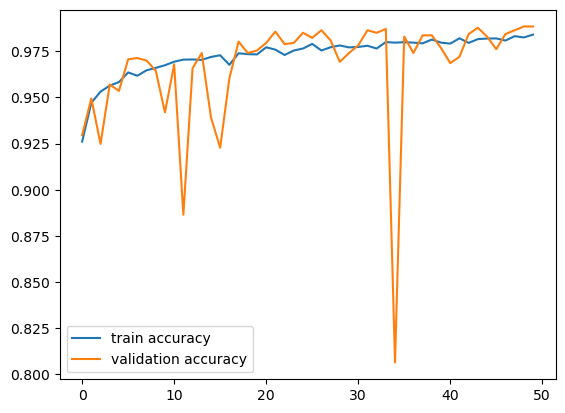
\includegraphics[width=0.785\textwidth]{\mypath/accuracy_pretrain.png}}
		\caption{Accuracy of model used for transfer learning during training}
	\end{figure}

	\begin{figure}[h!]
		\centerline{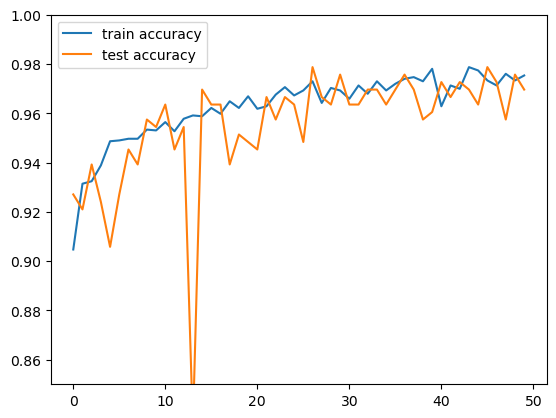
\includegraphics[width=0.785\textwidth]{\mypath/accuracy_basic.png}}
		\caption{Accuracy of model trained using only Masstrich data}
	\end{figure}

	\begin{figure}[h!]
		\centerline{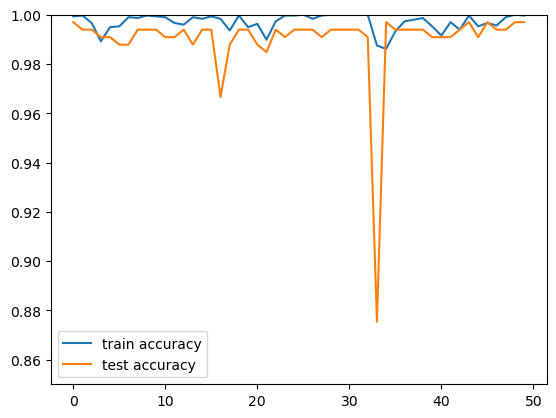
\includegraphics[width=0.785\textwidth]{\mypath/accuracy_transfer.png}}
		\caption{Accuracy of model trained using Masstrich data and pre-trained model}
	\end{figure}
	\newpage
	Examining the accuracy plots of our models, we observe that both the model later employed as the pre-trained model and the model trained exclusively on Maastricht data consistently increased accuracy throughout the entire training process. Notably, the accuracy of the pre-trained model is generally higher, likely attributable to its larger training dataset (approximately four times larger).
	\\
	
	Upon reviewing the accuracy plot for the model training only the last layer using Maastricht data and leveraging other layers from the pre-trained model, it becomes apparent that the accuracy remains consistently high throughout the entire training duration, with improvements appearing to be marginal.   
	\\
	
	If we compute validation accuracy using approximately 10\% of Maastrich data not used during training we get these values for our three models:
	\begin{table}[!h]
		\begin{tabular}{|l|l|}
			\hline
			model &  validation accuracy  \\ \hline
			Pre-trained on different cities  & 0.98356 \\ \hline
			Standard Neural Network & 0.97260 \\ \hline
			Trasfer learning using pre-trained &  0.99178 \\ \hline
		\end{tabular}
	\end{table} 

	The model used as the pre-trained model demonstrates slightly better results than the standard model, despite the disadvantage of never having encountered any data from Maastricht. Notably, our model employing transfer learning from the pre-trained model achieved the highest accuracy, suggesting that transfer learning indeed enhanced the model. However, due to high overall accuracy and the minimal differences in accuracy between these models, it is not appropriate to draw definitive conclusions.
	
	\newpage
	
	\section{Unsupervised learning - clustering}
	
	We will utilize four distinct clustering models with predominantly default settings, treating the task as unsupervised learning. In this approach, we refrain from leveraging labels to enhance the model but rather employ them solely for validation purposes.
	\\
	
	Here are model we will compare:
	\begin{itemize}
		\item K-Means Clustering (sklearn.cluster.KMeans) - standard K-means algorithm utilizing Lloyd's algorithm, which aims to minimize the sum of distances between each point and the center of the cluster to which it belongs
		\item Spectral Clustering (sklearn.cluster.SpectralClustering) - it involves computing the affinity matrix of points using an RBF kernel, followed by the generation of the Laplacian matrix from this affinity matrix. Finally, clusters are determined by applying the K-Means algorithm on the Laplacian projection of the points
		\item Agglomerative Clustering (sklearn.cluster.AgglomerativeClustering) - hierarchical clustering algorithm recursively merges pairs of clusters from sample data, aiming to minimize the variance within the clusters being combined using Euclidean distance 
		\item Gaussian Mixture (sklearn.mixture.GaussianMixture) - this model endeavors to represent each sample data point as originating from one of multiple Gaussian distributions. Initially, it employs the K-Means algorithm to partition the points, and subsequently optimizes their affiliation to Gaussian distributions using the Expectation-Maximization (EM) algorithm
	\end{itemize}

	We will apply these algorithms to datasets from three distinct cities: Budapest, Perpignan, and Dresden. The validation score is computed as the percentage of correctly "labeled" validation data points, with a mapping between clusters and labels designed to maximize the validation score (therefore a minimal score is 0.5). Additionally, we will compare our models with a baseline model that places all points into one cluster, assuming a uniform label for the entire dataset (majority label). Another baseline model worth considering is one that randomly assigns points to clusters. However, this model consistently attains a minimum possible score of 0.5 due to the mapping of clusters to labels. Therefore, we have opted not to include it in our analysis.
	\\
	
	Now let's look at results for each of our three cities:
	\\
	
	Budapest:
	\begin{table}[!h]
		\begin{tabular}{|l|l|}
			\hline
			model &  validation score  \\ \hline
			Base & 0.62466 \\ \hline
			K-Means Clustering & 0.89863 \\ \hline
			Spectral Clustering &  0.89315 \\ \hline
			Agglomerative Clustering  &  0.85479 \\ \hline
			Gaussian Mixture &  0.90137 \\ \hline
		\end{tabular}
	\end{table} 

	Upon comparison with the base model, it is evident that all other models exhibit significantly higher scores. With the exception of Agglomerative Clustering, all models achieve a score around 0.9, indicating an accuracy of 90\%. From this observation, we can infer that all our models effectively partition the data into clusters that align closely with their respective labeling.
	\\
	
	Perpignan:
	\begin{table}[!h]
		\begin{tabular}{|l|l|}
			\hline
			model &  validation score  \\ \hline
			Base & 0.53150 \\ \hline
			K-Means Clustering & 0.83836 \\ \hline
			Spectral Clustering &  0.51232 \\ \hline
			Agglomerative Clustering  &  0.79726 \\ \hline
			Gaussian Mixture &  0.82192 \\ \hline
		\end{tabular}
	\end{table} 

	In this comparison, the base model barely surpasses a score of 0.5, suggesting an approximately equal distribution of each label within our validation dataset. Evaluating the scores of clustering models reveals that three models markedly outperformed the base model. However, Spectral Clustering achieved a score close to the minimal possible, indicating that there is likely no discernible relationship between this clustering approach and the assigned labels.
	\\

	Dresden:
	\begin{table}[!h]
		\begin{tabular}{|l|l|}
			\hline
			model &  validation score  \\ \hline
			Base & 0.77808 \\ \hline
			K-Means Clustering & 0.77534 \\ \hline
			Spectral Clustering &  0.77260 \\ \hline
			Agglomerative Clustering  &  0.73424 \\ \hline
			Gaussian Mixture &  0.80822 \\ \hline
		\end{tabular}
	\end{table} 
	
	In this analysis, the base model exhibits a score of around 0.77, indicating a notable skewness towards one label value in the validation data for this city. Interestingly, all our models achieved scores close to that of the base model. Consequently, we cannot assert the superiority of any model over the base model in this specific scenario.
	\\
	
	In general, it appears that the most effective model for discerning whether weather is suitable for a picnic without explicitly labeled data is the Gaussian Mixture Model. Across all three cities, it consistently emerged as either the best or the second-best model. However, it's essential to note that in cases where the data is highly skewed towards one label, even this model may not be as informative or effective.
	\\
	
	Now, we aim to visualize our best and worst results. To achieve this, we'll employ the PCA algorithm to reduce our data to two dimensions and then visualize it using a scatter plot. The points in the plot will be colored according to their labels (clusters).
	\newpage
	So our best model was Gaussian Mixture model for Budapest data:
	
	\begin{figure}[h!]
		\centerline{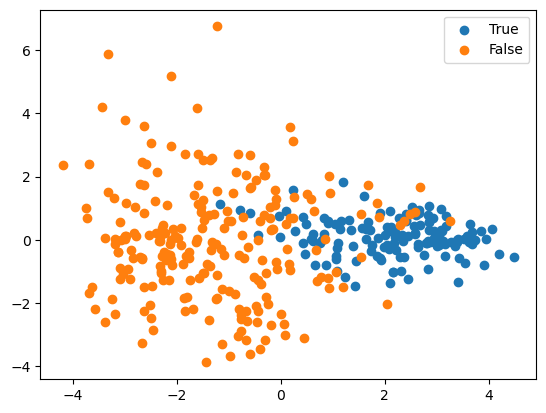
\includegraphics[width=0.7\textwidth]{\mypath/budapest_label.png}}
		\caption{Real split into weather suitable and not suitable for picnic in Budapest}
	\end{figure}
	
	\begin{figure}[h!]
		\centerline{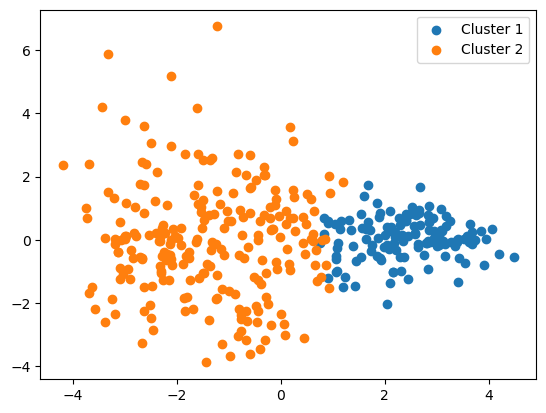
\includegraphics[width=0.7\textwidth]{\mypath/budapest_gauss.png}}
		\caption{Split into weather suitable and not suitable for picnic in Budapest using Gaussian Mixture model}
	\end{figure}

	he visual comparison reveals a distinct resemblance between these two splits. Notably, even after dimension reduction using PCA, the Gaussian Mixture model still distinctly delineates the borders between clusters. In contrast, the boundaries between the actual labels appear more ambiguous in the visualization, providing insight into why the model may not achieve 100\% accuracy.
	\\
	\newpage
	Our worst performing model was Spectral Clustering for Perpignan data that has score similar to either one cluster or random model.
	
	\begin{figure}[h!]
		\centerline{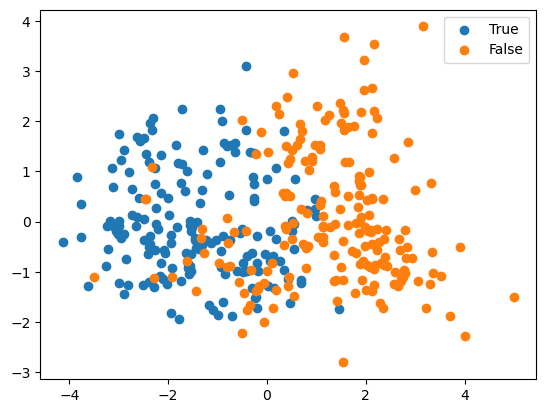
\includegraphics[width=0.70\textwidth]{\mypath/perpignan_label.png}}
		\caption{Real split into weather suitable and not suitable for picnic in Perpignan}
	\end{figure}
	
	\begin{figure}[h!]
		\centerline{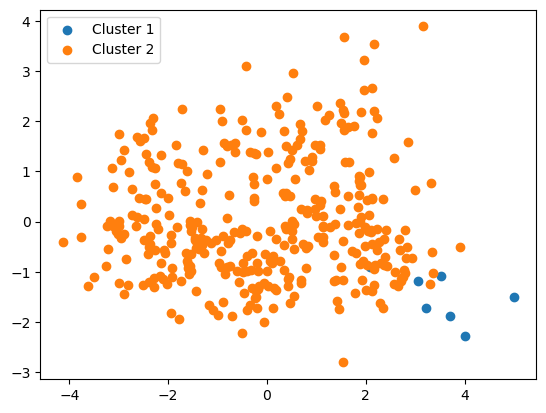
\includegraphics[width=0.70\textwidth]{\mypath/perpignan_spectral.png}}
		\caption{Split into weather suitable and not suitable for picnic in Perpignan using Spectral Clustering model}
	\end{figure}
	
	In this observation, the reason for the close proximity of the Spectral Clustering model to the base model with a single cluster becomes apparent—it forms one large cluster encompassing more than 98\% of the data points. Examining the actual labeling, we discern a vague border between the label groups. However, as indicated by the results from other models, there is a degree of success in approximating this border even without knowledge of the labels.
	
\end{document}